\documentclass[twocolumn,10pt]{article}
\usepackage[letterpaper,left=1.95cm,right=1.95cm,top=2.5cm,bottom=3.16cm]{geometry} % Márgenes y demás
\usepackage[utf8]{inputenc}
\usepackage{algpseudocode}
\usepackage{algorithm}
\usepackage{pxfonts}
\usepackage{wasysym} % symbols
\usepackage{amssymb} % symbols
\usepackage{abstract}
\usepackage{parskip}
\usepackage{float}
\PassOptionsToPackage{hyphens}{url}\usepackage[hidelinks]{hyperref}
\usepackage{tabularx}
%\def\sym##1{\ifmmode^{##1}\else\(^{##1}\)\fi}
\usepackage{titlesec}
\usepackage{xcolor}
\usepackage{hyperref}
\hypersetup
{
    colorlinks = false,
    linkbordercolor = {white}, citebordercolor = {white}
}
\usepackage{float}
\usepackage{graphicx}
\usepackage{blindtext}% only for dummy text
\usepackage{fancyhdr}
\usepackage{titling}
\usepackage{caption}
\captionsetup[table]{
  position=above,
  justification=raggedright,
  labelsep=newline, % <<< label and text on different lines
  singlelinecheck=false % <<< raggadright also when the caption is shorter
                        % than a single line
}
\usepackage[document]{ragged2e}
\usepackage[affil-sl]{authblk} 
\usepackage{mathptmx}  %Times new Roman

\setlength{\columnsep}{1cm}
\renewcommand{\refname}{BIBLIOGRAFÍA}
\renewcommand{\figurename}{Fig.}
\renewcommand{\tablename}{Tabla.}
\renewcommand{\abstractname}{RESUMEN}

% Keywords command
\providecommand{\keywordsSpan}[1]
{
  \small	
  \textbf{\textit{Palabras Clave:}} #1
}

\providecommand{\keywordsEng}[1]
{
  \small	
  \textbf{\textit{Keywords:}} #1
}


%%%%%%%% FORMATO DE LAS SECCIONES Y SUBSECCIONES %%%%%
\titleformat{\section} 
	{\normalfont\large\bfseries}{\makebox[30pt][l]{\thesection}}{0pt}{} 
\titleformat{\subsection} 
	{\normalfont\large\bfseries }{\makebox[30pt][l]{\thesubsection}}{0pt}{}
\renewcommand\thesection{\arabic{section}.}
\renewcommand\thesubsection{\thesection\arabic{subsection}}
%%%%%%%% FORMATO DE LAS SECCIONES Y SUBSECCIONES %%%%%


	
\makeatletter
\long\def\@makecaption#1#2{
\vskip\abovecaptionskip
\sbox\@tempboxa{#1. #2}
\ifdim \wd\@tempboxa >\hsize
#1. #2\par
\else
\global \@minipagefalse
\hb@xt@\hsize{\hfil\box\@tempboxa\hfil}
\fi
\vskip\belowcaptionskip}
\makeatother


\pagestyle{fancyplain}% <- pagestyle fancyplain
\fancyfoot[C]{}
\renewcommand\plainheadrulewidth{.4pt}% headrule on plain pages
%\fancyhf{}
\rhead{15 de noviembre del 2021}
\lhead{ Temas Selectos de Optimización Martes M4-M6 Grupo 001 }
\rfoot{\thepage}





%%%%%% CORRESPONSE AUTHOR %%%%%
\fancypagestyle{alim}
{
\fancyfoot[C]{}
\renewcommand\plainheadrulewidth{.4pt}% headrule on plain pages
%\fancyhf{}
\fancyhf{}\renewcommand{\headrulewidth}{0.4pt}
% \fancyfoot[R]{
% \textcolor{gray}{\textbf{How to cite}: Autor uno, Autor dos, Autor tres\\[0.1cm]
%     Título del artículo en español\\[0.1cm]
%     Revista EJE, Vol. \# No. \#, p1-pn, 20XX\\[0.1cm]
%     \textbf{DOI}: http://dx.doi.org/000.000.000
% }
% }
\fancyhead[R]{15 de noviembre del 2021}
\lhead{Temas Selectos de Optimización Martes M4-M6 Grupo 001 }
    \renewcommand\plainheadrulewidth{.4pt}% headrule on plain pages
}

%%%%%%%%%%%%%%%%%%%%%%%%%%%%%%%%%%

\date{}



  %%Llama el archivo de los estilos

%%%%%%% ENCABEZADO %%%%%%%%%%%%%%%%%%%%

{\title{\fontsize{16}{16}
\vspace*{-0.7cm}
\textbf{
Algoritmo Heurístico para un Problema de Secuenciación de Tareas
} \\[0.2cm]
\fontsize{12}{12}
\textbf{Heuristic Algorithm for Scheduling Problem
}\\[0.2cm]}
}

\author{\fontsize{10pt}{10pt}\selectfont \textbf{Eduardo Vicente Reyna Villela, Gonzalo Alberto Guajardo Galindo, \\Ely Federico Torres Rodríguez, Jorge Alberto Prado Rivas}
}



\affil{ 
\fontsize{8pt}{8pt}\selectfont Universidad Autónoma de Nuevo León, Facultad de Ingeniería Mecánica y Eléctrica \\ Av. Universidad S/N, Ciudad Universitaria San Nicolás de los Garza, N. L., C.P. 66455 } \fontsize{8}{8}



%%%%%%%%%%%%%%%%%%%%%%%%%%%%%%%%% INICIO DEL DOCUMENTO
%%%%%%%%%%%%%%%%%%%%%%%%%%%%%%%%%%%%%%%%%%%%%%%%%%%%%%%%%%%%%%%%%%%%%%%


\begin{document}
\twocolumn

\maketitle
\begin{abstract}
\vspace*{0.5cm}
\justify
\fontsize{10pt}{10pt}\selectfont
En este proyecto se presenta un problema de secuenciación de tareas con el objetivo de diseñar un algoritmo heurístico que encuentre la mejor solución para resolver la secuenciación de tareas que tiene una máquina que produce una cierta cantidad de productos minimizando los tiempos requeridos para procesarlas. El problema es resuelto utilizando la lógica del método del vecino más cercano en un problema TSP. En este reporte se muestran los pasos del algoritmo de implementación, así como la interpretación de los resultados que se obtuvieron.

\keywordsSpan{heurística, secuenciación, tareas, makespan, minimización, tiempo, producción, mantenimiento, periodo.}
\end{abstract}
\vspace{0.5cm}


\renewcommand{\abstractname}{ABSTRACT}
\begin{abstract}
\vspace*{0.5cm}
\justify

\textit{In this project, a task sequencing problem is presented with the aim of designing a heuristic algorithm that finds the best solution to solve the task sequencing of a machine that produces a certain amount of products while minimizing the time required to process them. The problem is solved by using the logic of the nearest neighbor method in a TSP problem. This report shows the steps of the implementation algorithm, as well as the interpretation of the results obtained.}

\keywordsEng{heuristics, sequencing, tasks, makespan, minimization, time, production, maintenance, period.}
\end{abstract}

\vspace*{0.5cm}  %%% Espacio entre el abstract y las columnas



\thispagestyle{alim}


\section{INTRODUCCIÓN}
\justifying
Mediante este documento se realiza un análisis y solución al problema de secuenciación de tareas, se consideran los problemas de scheduling en entornos single-machine (Una sola maquina), con indeterminación en el tiempo de procesamiento de los trabajos sin restricciones, la función objetivo consiste en minimizar el tiempo máximo de terminación de los procesos, también llamado makespan. Para resolver este problema, se propone un algoritmo en el cual la imprecisión en los tiempos de procesamiento de los trabajos se representa mediante números difusos y se utiliza una medida de comparación robusta que permite ordenar dichos números para así obtener la secuencia óptima. La mayoría de estos problemas de secuenciación son de optimización combinatoria y una gran parte de estos pertenecen a la clase de problemas NP-Hard. Los problemas NP-hard son un subconjunto de la clase de NP (problemas que no se puede tener una solución en tiempo para todas sus instancias) con la característica de que todos los problemas de esta clase pueden ser reducidos a él, los problemas para los que se puede encontrar un algoritmo de solución en tiempo polinomial forman la clase P, que es un subconjunto de la clase NP. Muchos problemas, que son NP-hard en general, pueden resolverse en tiempo polinomial en el caso de una sola máquina.
En este proyecto se plantea una metodología para solucionar el problema de Secuenciación de tareas a través de la aplicación de una técnica heurística, con la que se pretende establecer la secuencia de una sola maquina y a la vez optimizar una medida de efectividad que para este caso es minimizar el tiempo total requerido para la finalización de todas las tareas (makespan). El problema fue resuelto empleando el algoritmo heurístico del vecino más cercano.


\section{REVISIÓN DE LITERATURA}
El problema de secuenciación de tareas define los periodos de tiempo durante los cuales las maquinas pueden trabajar únicamente en un conjunto especifico de tareas configuradas como uno o más conjuntos de procesos. En este caso trabajaremos con el makespan que es el tiempo que transcurre entre el inicio del primer trabajo en la primera máquina y la terminación del último trabajo en la última máquina. Single-machine scheduling problema (SMSP) es uno de los problemas de programación clásicos más estudiados debido a su amplia gama de aplicaciones en muchos sistemas realistas y se aplica en las diferentes áreas donde se tienen como común denominador la asignación de tareas, la planificación de horizontes de trabajos y la optimización de las operaciones entre recursos y tareas, entre otros\cite{Ying}. 
Un Scheduling puede definirse como la tarea de determinar el inicio y finalización de cada operación (Alharkan, 2010) a ser procesada en un taller (fábrica, planta). Al resultado de esta planificación se le denomina Schedule (secuencia de trabajos) que puede ser, por ejemplo, un horario, planes de aterrizaje o de despegue de aviones, atraques de barcos, etc. Desde el punto de vista matemático, puede entenderse como un arreglo de trabajos y operaciones que deben satisfacer ciertas condiciones de asignación y restricciones, además de satisfacer una condición de la optimalidad en los resultados\cite{Senthilkumar}.
El algoritmo del agente viajero (Travelling Salesman Problem) es un problema que consiste en encontrar el circuito óptimo (en términos del viaje más corto) que deberá seguir un vendedor en un caso con n ciudades, en el que cada ciudad se visita exactamente una vez. Básicamente es una adaptación del Problema de Asignación que considera restricciones adicionales que garantiza la exclusión de subcircuitos en la solución óptima\cite{GeeksforGeeks}.
El algoritmo del vecino más cercano (Nearest Neighbor Algorithm) es un algoritmo que simplemente busca en las observaciones más cercanas a la que se está tratando de predecir y clasifica el punto de interés basado en la mayoría de los datos que le rodean. Es una heurística miope, es decir, en una iteración escoge la mejor opción que tiene disponible, sin ver que esto puede obligarle a tomar malas decisiones posteriormente; al final del proceso probablemente quedaran vértices cuya conexión obligar a introducir aristas de coste elevado.


\section{DEFINICIÓN DEL PROBLEMA}
La secuenciación de tareas consiste en programar de forma óptima un conjunto de N tareas en una máquina, considerando que todas las tareas tienen el mismo orden de procesamiento, los tiempos de ejecución varían en los productos, se consideran tiempos de preparación de la maquina entre una tarea y otra, este tiempo de preparación es necesario para cambio de herramienta, material, etc. Se debe tener una etapa de mantenimiento M cada cierto periodo de tiempo T y los trabajos no pueden ser interrumpidos. El objetivo es la minimización del tiempo requerido para terminar todas las tareas o makespan de lo cual resulta la secuencia optima de procesamiento de todas las tareas\cite{Gupta}.



\subsection{MODELO MATEMÁTICO}
La premisa del modelo matemático es contar con una función objetivo que minimice el makespan, es decir el tiempo total en el que se encuentre operando la máquina para producir todos los productos existentes, a través de esto se tienen diferentes restricciones, la primera de ellas es que existe un periodo de tiempo T que no debe sobrepasarse ya que se necesita de un tiempo de mantenimiento para cada periodo de tiempo T y para lograr esto todos los bienes deben producirse hasta su totalidad sin dejar ninguno en estado pendiente.




Tp significa tiempo de producción, y es el tiempo en que se tardan en producir todos los productos, por otra parte se está multiplicando la variable $\:c_{ij}$ que es el costo de que se procese el producto $j$ después del producto $i$ por la variable $\:x_{ij}$ que toma el valor de 1 si el producto $j$ se procesa después del producto $i$, esto se puede observar en la ecuación 1
\begin{equation}
min\:\:Tp\:+\sum \:_{i\:=\:0}^n\:\sum \:_{j\:=\:1}^n\:c_{ij}\:x_{ij}
\end{equation}



\section{MÉTODO DE SOLUCIÓN PROPUESTO}
Para la resolución del problema, lo que se llevó a cabo fue seguir el método del $Nearest Neighbor Algorithm$ Por medio de este algoritmo lo que se trata es tomar en cuenta la matriz de tiempos de preparación, es decir el tiempo que toma de pasar de un producto que se acaba de procesar a uno que empezará a procesarse.





\subsection{ALGORITMO DEL PROGRAMA}
A continuación se muestra un pseudocódigo que inicia con la lectura de los datos de las instancias que incluye el número de productos, tiempo del mantenimiento M, tiempo del periodo T, tiempos de producción y la matriz de tiempos de preparación, después de esto inicia el primer periodo de tiempo, y mientras aún falten productos por agregar a la secuencia, se buscará el producto que tenga el menor tiempo de preparación, en el caso de que se pase del tiempo límite del periodo, se empezará uno nuevo, al final se arrojan los resultados del algoritmo.
\begin{algorithm}
\caption{Menor tiempo de preparación}\label{alg:cap}
\begin{algorithmic}
\State Lectura de datos
\State Se inicia un periodo de tiempo T
\While{siga faltando productos}
\State Buscar producto con menor tiempo de preparación
\If{no se pasa del tiempo límite}
    	\State Se agrega a la secuencia
\Else{}
    	\State Se agrega el tiempo de mantenimiento M
    	\State Se inicia un nuevo periodo de tiempo T. 
	\State Ir al paso 2
\EndIf
\EndWhile
\State Calcular makespane de la secuencia final
\State Arrojar secuencia final y makespan
\end{algorithmic}
\end{algorithm}





\section{EXPERIMENTACIÓN \\COMPUTACIONAL}

Se desarrolló el algoritmo a través del lenguaje de programación Python, se utilizaron varias librerías entre las que se encuentran numpy y pandas para hacer la lectura de los datos y facilitarnos el trabajo al momento de extraer la información desde un archivo externo.En total se realizó la prueba del algoritmo en 4 instancias, la primera de 10 productos, la segunda de 20 productos y por último la tercera y cuarta con el mismo número de productos, en este caso de 50 se realizó la ejecución del programa para estas 4 instancias, se imprimieron los datos obtenidos de los archivos externos para la generación de las tablas de datos, así como los resultados que arrojó el programa.
 


\subsection{INSTANCIA I}
\textbf{Datos}\\
Trabajando con:  Instancia1.10.txt\\
No. de productos: 10\\
Tiempo de Mantenimiento M: 50\\
Tiempo de Periodo T: 300\\
Capacidad maxima C: 250

\begin{table}[h!]
\centering
\begin{tabular}{||c c||} 
 \hline
  &0 \\
\hline
   
0    &50\\
1   & 86\\
2   & 78\\
3   & 64\\
4  &  22\\
..  &...\\
6  &  82\\
7  &  87\\
8  &  52\\
9   &100\\
10  & 99\\
\hline

\end{tabular}
\caption{Columna de producción - Instancia 1}
\label{table:1}
\end{table}



\begin{table}[!h]
\centering
\begin{tabular}{||c c c c c c c c c c||} 
 \hline
  &0 &  1 &  2 &  3  & ... & 7  & 8 &  9  & 10\\
\hline
    
0 	&   0	&  8 	& 15  	& 7 	& ... 	& 14 	& 20  	&14  	& 9\\
1  	&  7  	& 0 	& 14	&  17 	& ... 	& 14 	& 14 	& 18  	& 8\\
2 	&   9 	& 11 	&  0  	&16 	& ...  	& 5 	& 10  	&11  	&18\\
3  	& 13 	& 18 	&  6  	& 0 	& ... 	& 19 	& 12	& 10	&  14\\
.. 	& .. 	& .. 	& .. 	& ..  	&...  	&..  	&..  	&.. 		& ..\\
7   	& 5 	& 15	&  12	&  5 	& ... 	&  0 	&12 	&  7  	&15\\
8 	&  5 	& 11  	& 8 	& 13 	& ... 	& 20 	&  0	&  18 	& 15\\
9  	&  7 	&  6 	& 14 	& 14 	& ... 	&  7 	& 16 	&  0  	& 7\\
10  & 6		&  11 	&  9 	& 18 	& ... 	& 15	&  18	&  20 	& 0\\
\hline

\end{tabular}
\caption{Matriz de preparación - Instancia 1}
\label{table:1}
\end{table}


\textbf{Resultados}\\
Secuencia de productos\\
3, 2, 0, 1, 10, 0, 6, 8, 0, 7, 4, 0, 9, 5, 0\\
Tiempo total\\
1160\\
De igual forma se realizó de forma manual la solución los datos de la Instancia 1 y efectivamente se obtuvieron los mismos, demostrando que el algoritmo funciona correctamente, en la Figura 1 se puede observar la solución gráfica.


\begin{figure}[!htb]
	\centering
	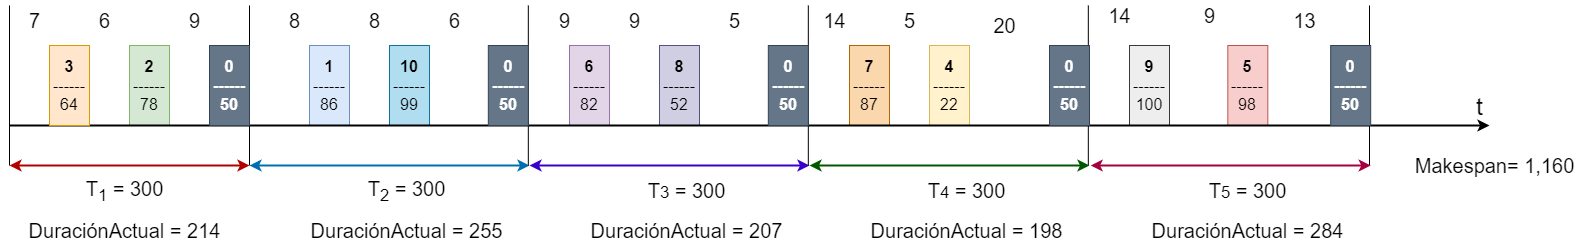
\includegraphics[width=8cm]{Figuras/Imagen1.png}
      \caption{Solución gráfica de la Instancia I}
      \label{fig:Instancia1_Fig}
\end{figure}







\subsection{INSTANCIA II}


\textbf{Datos}\\
Trabajando con:  Instancia1.20.txt\\
No. de productos: 20\\
Tiempo de Mantenimiento M: 30\\
Tiempo de Periodo T: 1000\\
Capacidad maxima C: 970\\



\begin{table}[h]
\centering
\begin{tabular}{||c c||} 
 \hline
  &0 \\
\hline
   
0   & 30\\
1  & 155\\
2  & 154\\
3  & 139\\
4  & 119\\
..  &...\\
16 &  93\\
17 & 177\\
18&  182\\
19&  190\\
20 & 114\\
\hline

\end{tabular}
\caption{Columna de producción - Instancia 2}
\label{table:1}
\end{table}







\begin{table}[H]
\centering
\begin{tabular}{||c c c c c c c c c c||} 
 \hline
  &0 &  1 &  2 &  3  & ... & 17  & 18 &  19  & 20\\
\hline
    
0  &  0 & 36 & 23 & 16  &... & 44 & 39 & 15 & 34\\
1  & 19  & 0 & 10  &15  &...  &40 & 31 & 37 & 38\\
2  & 40 & 28 &  0  &39  &... & 17 & 31 & 16 & 13\\
3  & 23 & 37 & 39 &  0 & ... & 40 & 12 & 13 & 37\\
.. & ..  &.. & ..&  ..&  ... & ..  &..&  .. & ..\\
17 & 30 & 18 & 39  &33 & ... & & 0  41 & 19 & 42\\
18 & 41 & 13 & 17  &25 & ... & 15 &  0&  35 & 29\\
19 & 14 & 35 & 13&  16 & ... & 36&  21  & 0 & 11\\
20  &40 & 17 & 28&  43 & ... & 32 & 13 &29  & 0\\
\hline

\end{tabular}
\caption{Matriz de preparación - Instancia 2}
\label{table:1}
\end{table}

\textbf{Resultados}\\
Secuencia de productos\\
19, 9, 16, 3, 6, 0, 7, 5, 17, 11, 20, 13, 8, 0, 14, 12, 2, 15, 10, 0, 4, 18, 1, 0\\
Tiempo total\\
3297





\subsection{INSTANCIA III}


\textbf{Datos}\\
Trabajando con:  Instancia1.50a.txt\\
No. de productos: 50\\
Tiempo de Mantenimiento M: 50\\
Tiempo de Periodo T: 4500\\
Capacidad maxima C: 4450\\



\begin{table}[h!]
\centering
\begin{tabular}{||c c||} 
 \hline
  &0 \\
\hline
   
0&50\\
1&53\\
2&126\\
3&75\\
4&131\\
..&...\\
46&93\\
47&117\\
48&116\\
49&74\\
50&93\\

\hline

\end{tabular}
\caption{Columna de producción - Instancia 3}
\label{table:1}
\end{table}



\begin{table}[h!]
\centering
\begin{tabular}{||c c c c c c c c c c||} 
 \hline
  &0 &  1 &  2 &  3  & ... &47&  48&  49&  50\\  
\hline
    
0& 0&18&34&31&...&41&21&37&33\\
1&19&0&15&23&...&22&28&23&37\\
2&34&26&0&34&...&13&22&40&29\\
3&40&17&27&0&...&19&14&36&40\\
..&..&..&..&..&...&..&..&..&..\\
47&22&39&11&36&...&0&37&40&41\\
48&15&36&45&26&...&21&0&22&22\\
49&37&36&16&19&...&20&11&0&30\\
50&25&29&37&30&...&30&30&42&0\\

\hline

\end{tabular}
\caption{Matriz de preparación - Instancia 3}
\label{table:1}
\end{table}


\textbf{Resultados}\\
Secuencia de productos\\
17, 23, 20, 16, 11, 38, 25, 47, 19, 18, 37, 26, 1, 45, 32, 28, 7, 15, 24, 5, 31, 3, 33, 8, 4, 12, 27, 21, 41, 22, 50, 9, 48, 34, 35, 6, 14, 44, 30, 29, 43, 0, 13, 40, 39, 46, 42, 2, 10, 49, 36, 0
Tiempo total\\
5491


\subsection{INSTANCIA IV}


\textbf{Datos}\\
Trabajando con:  Instancia1.50b.txt\\
No. de productos: 50\\
Tiempo de Mantenimiento M: 50\\
Tiempo de Periodo T: 500\\
Capacidad maxima C: 450\\



\begin{table}[h!]
\centering
\begin{tabular}{||c c||} 
 \hline
  &0 \\
\hline
   
0& 50\\
1&123\\
2& 87\\
3&128\\
4&136\\
..&...\\
46&80\\
47&52\\
48&147\\
49&116\\
50&140\\


\hline

\end{tabular}
\caption{Columna de producción - Instancia 4}
\label{table:1}
\end{table}

\begin{table}[h!]
\centering
\begin{tabular}{||c c c c c c c c c c||} 
 \hline
  &0 &  1 &  2 &  3  & ... &47&  48&  49&  50\\  
\hline
    
0& 0&43&16&13&...&36&40&38&17\\
1&14&0&42&12&...&33&21&21&17\\
2&45&17&0&40&...&11&26&15&27\\
3&37&28&44&0&...&33&39&17&25\\
..&..&..&..&..&...&..&..&..&..\\
47&35&36&11&40&...&0&45&14&37\\
48&40&15&34&28&...&19&0&30&32\\
49&30&17&44&43&...&35&19&0&20\\
50&21&14&11&25&...&31&15&19&0\\


\hline

\end{tabular}
\caption{Matriz de preparación - Instancia 4}
\label{table:1}
\end{table}

\textbf{Resultados}\\
Secuencia de productos\\
46, 1, 6, 0, 3, 10, 27, 20, 0, 26, 40, 9, 0, 38, 22, 33, 0, 44, 30, 14, 0, 2, 34, 35, 0, 50, 21, 32, 43, 0, 19, 18, 39, 45, 0, 42, 11, 36, 31, 
0, 16, 13, 29, 0, 7, 49, 37, 0, 4, 28, 41, 0, 17, 15, 0, 23, 12, 5, 0, 8, 47, 25, 0, 24, 48, 0\\
Tiempo total\\
6926


\section{ENLACE AL VIDEO PRESENTACIÓN}

A continuación se anexa al documento un enlace que redirige al origen de un vídeo que explica a través de una presentación lo mostrado en este reporte \url{www.videopresentacion.com}


\twocolumn
[
\begin{@twocolumnfalse}
\section{CONCLUSIONES}

Se logró poder dar una solución buena para cada una de las instancias, para este trabajo se realizaron 2 heurísticas, y se escogió la que mejores resultados arrojaron, la primera que fue la que mejor comportamiento tuvo durante las ejecuciones del programa, fue el Algoritmo 1, que sólo tomaba como valor mínimo los tiempos de preparación, es decir el tiempo que necesita para pasar de un producto que ya se procesó a otro que sigue por procesarse, este tiempo fue el que se tomó, la otra alternativa era realizar una matriz de cocientes de la división entre el tiempo de producción y el tiempo de preparación y de ahí tomar el producto que menor tiempo promedio le tome.
Con este trabajo se pudo entender un poco más acerca de las aplicaciones en las que se puede facultar la materia de Investigación de Operaciones, a través de una metodología que inicia con el diseño de un algoritmo que permita arrojar resultados quizás no excelente, pero sí buenos que se puedan obtener a través de un tiempo de ejecución adecuado en cuánto a los requerimientos en exigencia que se tengan.




\bibliographystyle{ieeetr}
\bibliography{Bibliografia}

\end{@twocolumnfalse}
]

\end{document}
